The full analysis is performed on 192 $\pm$ 8 $\ipb$ of integrated luminosity, as a 
preparation for larger luminosity scenarios in the near future.

The estimation of the background follows the strategies described in 
Section~\ref{sec:backgrounds}. We summarize here the yields for the main background
components. For $\dyll$, top and $\Wjets$ backgrounds, we report the 
expected yields after the $\WW$ selection, those results are then extrapolated 
to each Higgs signal mass point.

The expected contributions from $\dyll$ events outside the $Z$-mass region in data 
can be estimated by counting the number of events near the $Z$ mass region in data, 
subtracting from it the non-$Z$ contributions, and scaling it by a ratio $R_{out/in}$ 
defined as the fraction of events outside and inside the $Z$-mass region in the 
simulation. This procedure is applied separately to all jet bins. Electrons and muons 
are considered separately. The predictions for the three jet bins are shown in 
Tables~\ref{tab:dyestmm} and~\ref{tab:dyestee}.

%%%%%%%%%%%%%%%%%%%%%%%%%%%%%%
\begin{table}
\begin{center}
\begin{tabular}{l c c c}
\hline
Sample                                 &   0-jet             & 1-jet & 2-jet        \\
\hline
$R_{out/in}$ (simulation)              &   0.16 $\pm$ 0.01 $\pm$ 0.08 & 0.22 $\pm$ 0.01 $\pm$ 0.11 & 0.18 $\pm$ 0.02 $\pm$ 0.09	\\
$\mu\mu$ evens with $Z$-mass region    &         27        	      &       19		   &	 48			\\
$e\mu$ events with $Z$-mass region     &          9        	      &        7		   &	  2			\\
$\dymm+X$ simulation Prediction        &   0.89 $\pm$ 0.21 	      & 1.15 $\pm$ 0.23 	   & 3.57 $\pm$ 0.54		\\
Data-driven $\dymm+X$ Estimate         &   3.68 $\pm$ 0.84 $\pm$ 1.84 & 3.55 $\pm$ 0.99 $\pm$ 1.78 & 8.56 $\pm$ 1.26 $\pm$ 4.28 \\ 
\hline
\end{tabular}
\end{center}
\caption{Predictions of the off-peak $\dymm+X$ contribution compared 
with observed event counts in the data-driven estimation. The events are required to pass all 
$\WW$ selections. We report the statistical and systematic uncertainties for the data-driven estimate.}
\label{tab:dyestmm}
\end{table}
%%%%%%%%%%%%%%%%%%%%%%%%%%%%%%
\begin{table}
\begin{center}
\begin{tabular}{l c c c}
\hline
Sample                                 &   0-jet             & 1-jet & 2-jet        \\
\hline
$R_{out/in}$ (simulation)              &   0.13 $\pm$ 0.01 $\pm$ 0.07 & 0.19 $\pm$ 0.01 $\pm$ 0.10 & 0.15 $\pm$ 0.02 $\pm$ 0.08	\\
$ee$ evens with $Z$-mass region        &         14        	      &       11		   &	 28			\\
$e\mu$ events with $Z$-mass region     &          9        	      &        7		   &	  2			\\
$\dyee+X$ simulation Prediction        &   0.97 $\pm$ 0.13 	      & 0.72 $\pm$ 0.20 	   & 2.01 $\pm$ 0.39		\\
Data-driven $\dyee+X$ Estimate         &   1.15 $\pm$ 0.57 $\pm$ 0.58 & 1.32 $\pm$ 0.71 $\pm$ 0.66 & 4.10 $\pm$ 0.82 $\pm$ 2.05 \\ 
\hline
\end{tabular}
\end{center}
\caption{Predictions of the off-peak $\dymm+X$ contribution compared 
with observed event counts in the data-driven estimation. The events are required to pass all 
$\WW$ selections. We report the statistical and systematic uncertainties for the data-driven estimate.}
\label{tab:dyestee}
\end{table}
%%%%%%%%%%%%%%%%%%%%%%%%%%%%%%

The top tagging algorithm is used to both reject $\ttbar$ and $tW$ processes, 
and to estimate the residual contributions of these backgrounds, as explained in 
Section~\ref{sec:sel_toptag}. The MC prediction for the top background contribution is 
compared with observed event counts in the data-driven estimation,
as summarized in Table~\ref{tab:dyest_nomet}.

%%%%%%%%%%%%%%%%%%%%%%%%%%%%%%
\begin{table}
\begin{center}
\begin{tabular}{l c c c}
\hline
Sample                                        &   0-jet           & 1-jet           & 2-jet               \\
\hline
Estimated top events in simulation  	      &   7.55 $\pm$ 0.45 & 18.63 $\pm$ 1.33& 18.12 $\pm$ 0.72	  \\
tagging efficiency (\%)                       &    56  $\pm$  7   &  69  $\pm$ 3    &  69  $\pm$  3	  \\
top-tagged events in data           	      &          22       &       53        &        45  	  \\
Data-driven top background estimate           &  14.37 $\pm$ 5.34 & 21.90 $\pm$ 4.70& 18.39 $\pm$ 4.11    \\
\hline
\end{tabular}
\end{center}
\caption{Predictions of the top background contribution compared 
with observed event counts in the data-driven estimation. The uncertainties are 
statistical only. The method is dominated by the available data in the control regions, 
hence any possible uncertainty on the method does not add anything significant.}
\label{tab:dyest_nomet}
\end{table}
%%%%%%%%%%%%%%%%%%%%%%%%%%%%%%

The estimation of the fake leptons from $\Wjets$ is explained in 
Section~\ref{sec:bkg_fakes}. The event predictions in the 0-jet, 1-jet 
and 2-jet bins are 25.19 $\pm$ 1.93 $\pm$ 7.56, 11.04 $\pm$ 1.34 $\pm$ 3.31 and 
3.02 $\pm$ 0.75 $\pm$ 0.91, respectively.

As a summary, the expected number of signal and background events after 
applying the $\WW$ selection requirements for each jet bin are shown in 
Table~\ref{tab:wwselection_all}. The extrapolation from the $\WW$ region 
to each $H \to \WW$ region of all the non-$\WW$ background is obtained from simulated 
events taking into account the previously computed scale factors.

\begin{table}[!ht]
  \begin{center}
 {\small
  \begin{tabular} {|c|c|c|c|c|c|}
\hline
          &   data & all bkg. & $qq \to \WW$ & $gg \to \WW$ &  $\ttbar+tW$ \\
  \hline
  \hline
 0-jet &  130 & 119.7 $\pm$  2.4  & 67.3 $\pm$ 0.3 &  3.4 $\pm$   0.1 &  14.3 $\pm$ 0.8 \\
 1-jet &   67 &  61.2 $\pm$  2.1  & 19.1 $\pm$ 0.2 &  1.1 $\pm$   0.1 &  21.9 $\pm$ 1.4 \\
 2-jet &   43 &  40.1 $\pm$  3.6  &  4.1 $\pm$ 0.1 &  0.2 $\pm$   0.1 &  18.3 $\pm$ 0.8 \\
 \hline
 \hline
  \end{tabular}
  \begin{tabular} {|c|c|c|c|c|}
\hline
       & non-resonant $WZ$/$ZZ$ & $\dyll+WZ+ZZ$ & $\Wjets$& $W+\gamma$ \\
  \hline
  \hline
 0-jet &   1.8 $\pm$	0.1 &  5.6 $\pm$   1.1 & 25.2 $\pm$   1.9 & 2.1 $\pm$   0.3  \\
 1-jet &   1.4 $\pm$	0.1 &  6.2 $\pm$   1.4 & 11.0 $\pm$   1.3 & 0.4 $\pm$   0.1 \\
 2-jet &   0.3 $\pm$	0.1 & 14.1 $\pm$   3.4 &  3.0 $\pm$   0.7 & 0.4 $\pm$   0.1 \\
 \hline
 \hline
  \end{tabular}
  }
  \caption{Expected number of signal and background events from the data-driven methods for an 
  integrated luminosity of 192 $\ipb$ after applying the $\WW$ selection requirements. 
  Only the statistical uncertainty on the samples is reported.}
   \label{tab:wwselection_all}
  \end{center}
\end{table}

The $\WW$ background estimation procedure defined in Section~\ref{sec:bkg_ww} is applied on the 
collected data. In the $\WW$ control region, the top and fake backgrounds are estimated from data, while the 
others are taken from MC. For the 0- and 1-jet bin analyses we find results consistent with 
expectations for $m_H$=120-200 $\GeVcc$, see Table~\ref{tab:wwEstimResData}. The procedure is 
not applied for $m_H>$200 $\GeVcc$ since the $\WW$ control region is expected to be significantly 
contaminated by Higgs events. 
For the 2-jet bin case the data luminosity is too small and yields are taken from the simulation.

\begin{table}[!htbp]
\begin{center}
\begin{tabular}{|c|c|c|c|c|} \hline
 & \multicolumn{2}{|c|}{0-jet bin} & \multicolumn{2}{|c|}{1-jet bin} \\ \hline
$m_H~[\GeVcc]$ & $\WW$ estimation & $\WW$ expected & $\WW$ estimation & $\WW$ expected \\ \hline
115 & 6.8 $\pm$ 2.0 & 6.47 $\pm$ 0.09 & 1.6 $\pm$ 1.2 & 1.35 $\pm$ 0.04 \\
120 & 8.6 $\pm$ 2.5 & 8.23 $\pm$ 0.10 & 2.0 $\pm$ 1.6 & 1.74 $\pm$ 0.04 \\
130 & 9.5 $\pm$ 2.7 & 9.00 $\pm$ 0.10 & 2.2 $\pm$ 1.7 & 1.93 $\pm$ 0.05 \\
140 & 8.5 $\pm$ 2.5 & 8.11 $\pm$ 0.10 & 1.9 $\pm$ 1.5 & 1.73 $\pm$ 0.04 \\
150 & 5.3 $\pm$ 1.6 & 5.41 $\pm$ 0.08 & 1.7 $\pm$ 1.5 & 1.60 $\pm$ 0.04 \\
160 & 3.8 $\pm$ 1.1 & 3.81 $\pm$ 0.06 & 1.4 $\pm$ 1.3 & 1.34 $\pm$ 0.04 \\
170 & 3.3 $\pm$ 1.0 & 3.25 $\pm$ 0.06 & 1.7 $\pm$ 1.4 & 1.54 $\pm$ 0.04 \\
180 & 4.3 $\pm$ 1.3 & 4.25 $\pm$ 0.06 & 2.0 $\pm$ 2.0 & 2.11 $\pm$ 0.05 \\
190 & 7.1 $\pm$ 2.1 & 6.90 $\pm$ 0.09 & 3.4 $\pm$ 3.0 & 3.24 $\pm$ 0.06 \\
200 & 7.5 $\pm$ 2.3 & 7.50 $\pm$ 0.09 & 3.8 $\pm$ 3.4 & 3.60 $\pm$ 0.06 \\  \hline
\end{tabular}
\caption{Data driven $WW$ estimation for different Higgs mass analyses in the 0- and 1-jet bins ($192~pb^{-1}$). 
Only statistical uncertainties are reported.}
\label{tab:wwEstimResData}
\end{center}
\end{table}

The cut based and multivariate analyses upper limits at 95\% C.L. are shown in 
Tables~\ref{fig:cutbase_uls_data} and~\ref{fig:mvabase_uls_data}, respectively. With 192 
$\ipb$ of data the upper limit is about 0.9 times the expectation of a Higgs boson of 
160~$\GeVcc$.

\begin{figure}[!htbp]
\begin{center}
   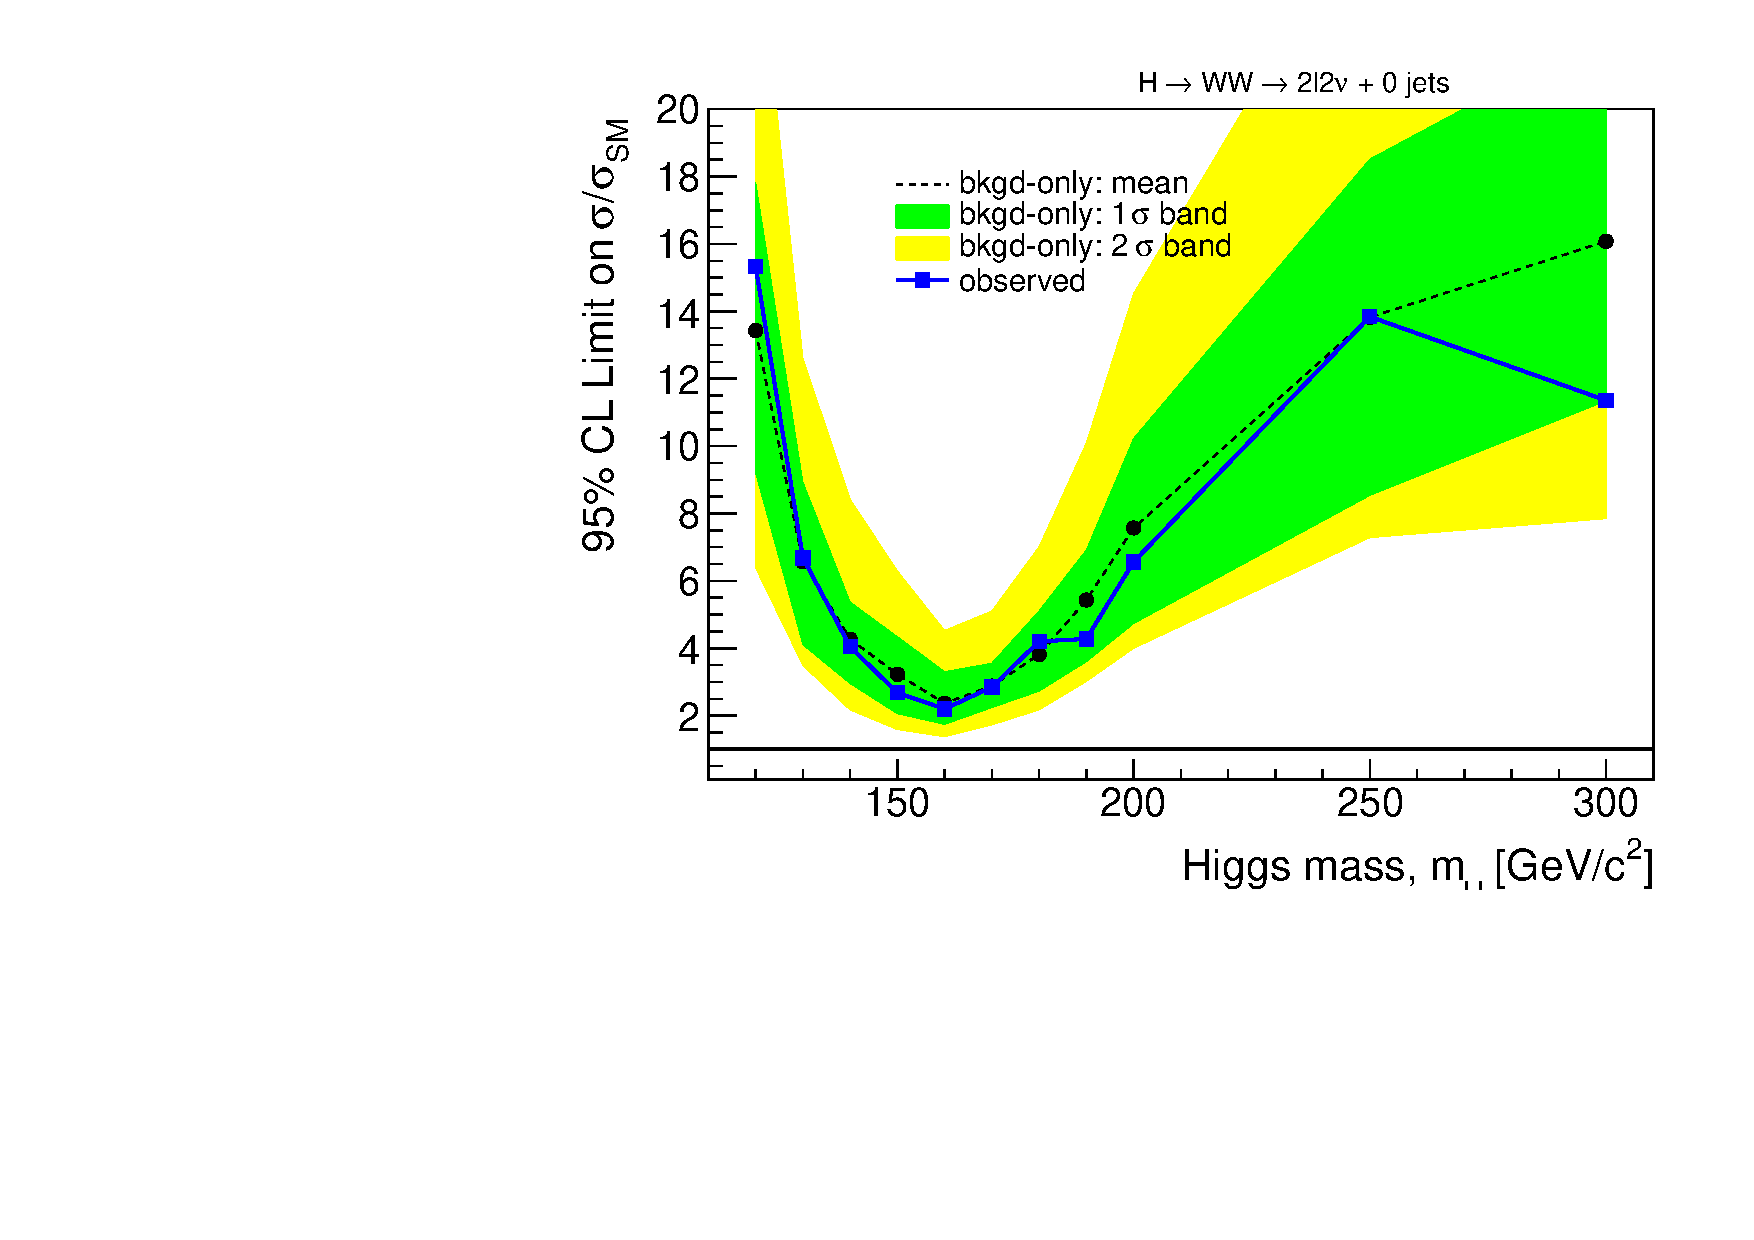
\includegraphics[width=0.49\textwidth]{figures/limits_0j_50pb_cut_1.pdf}
   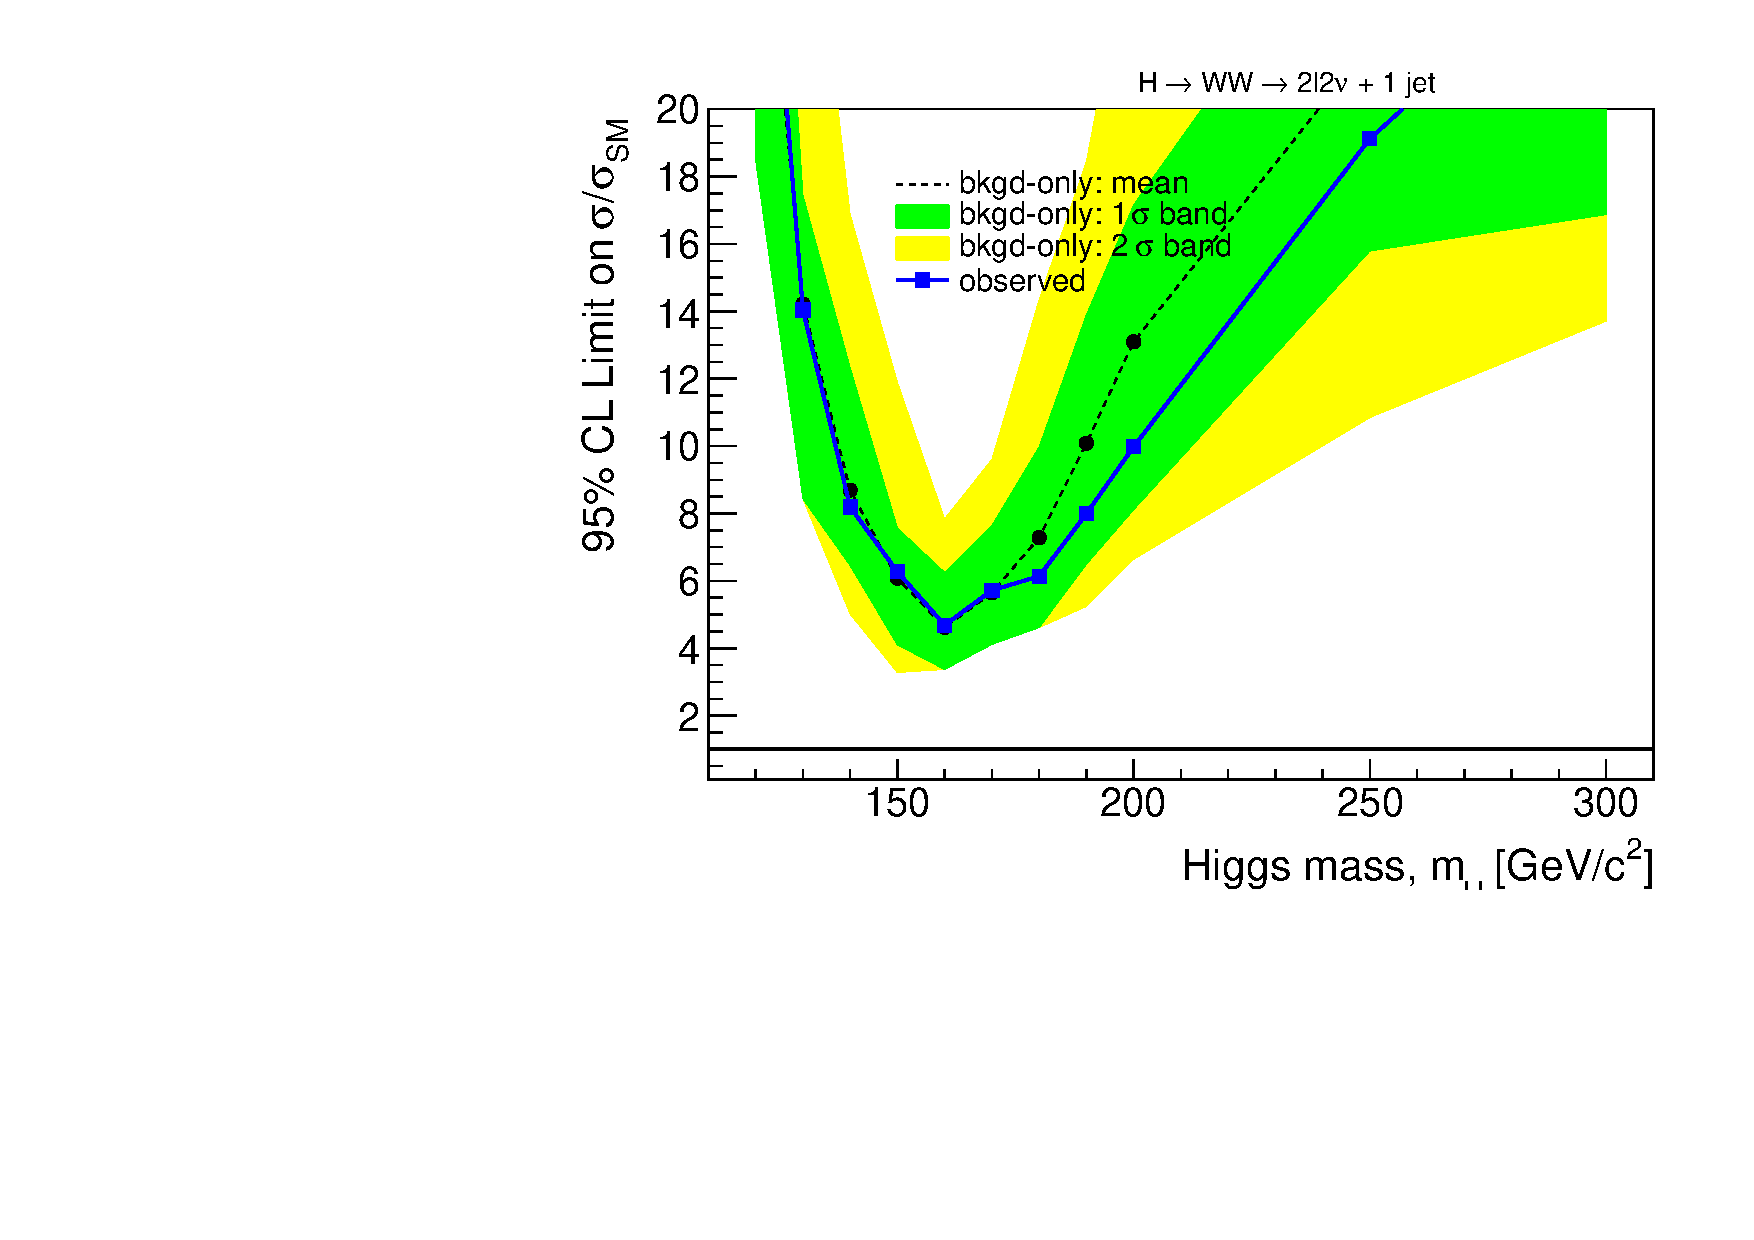
\includegraphics[width=0.49\textwidth]{figures/limits_1j_50pb_cut_1.pdf}
   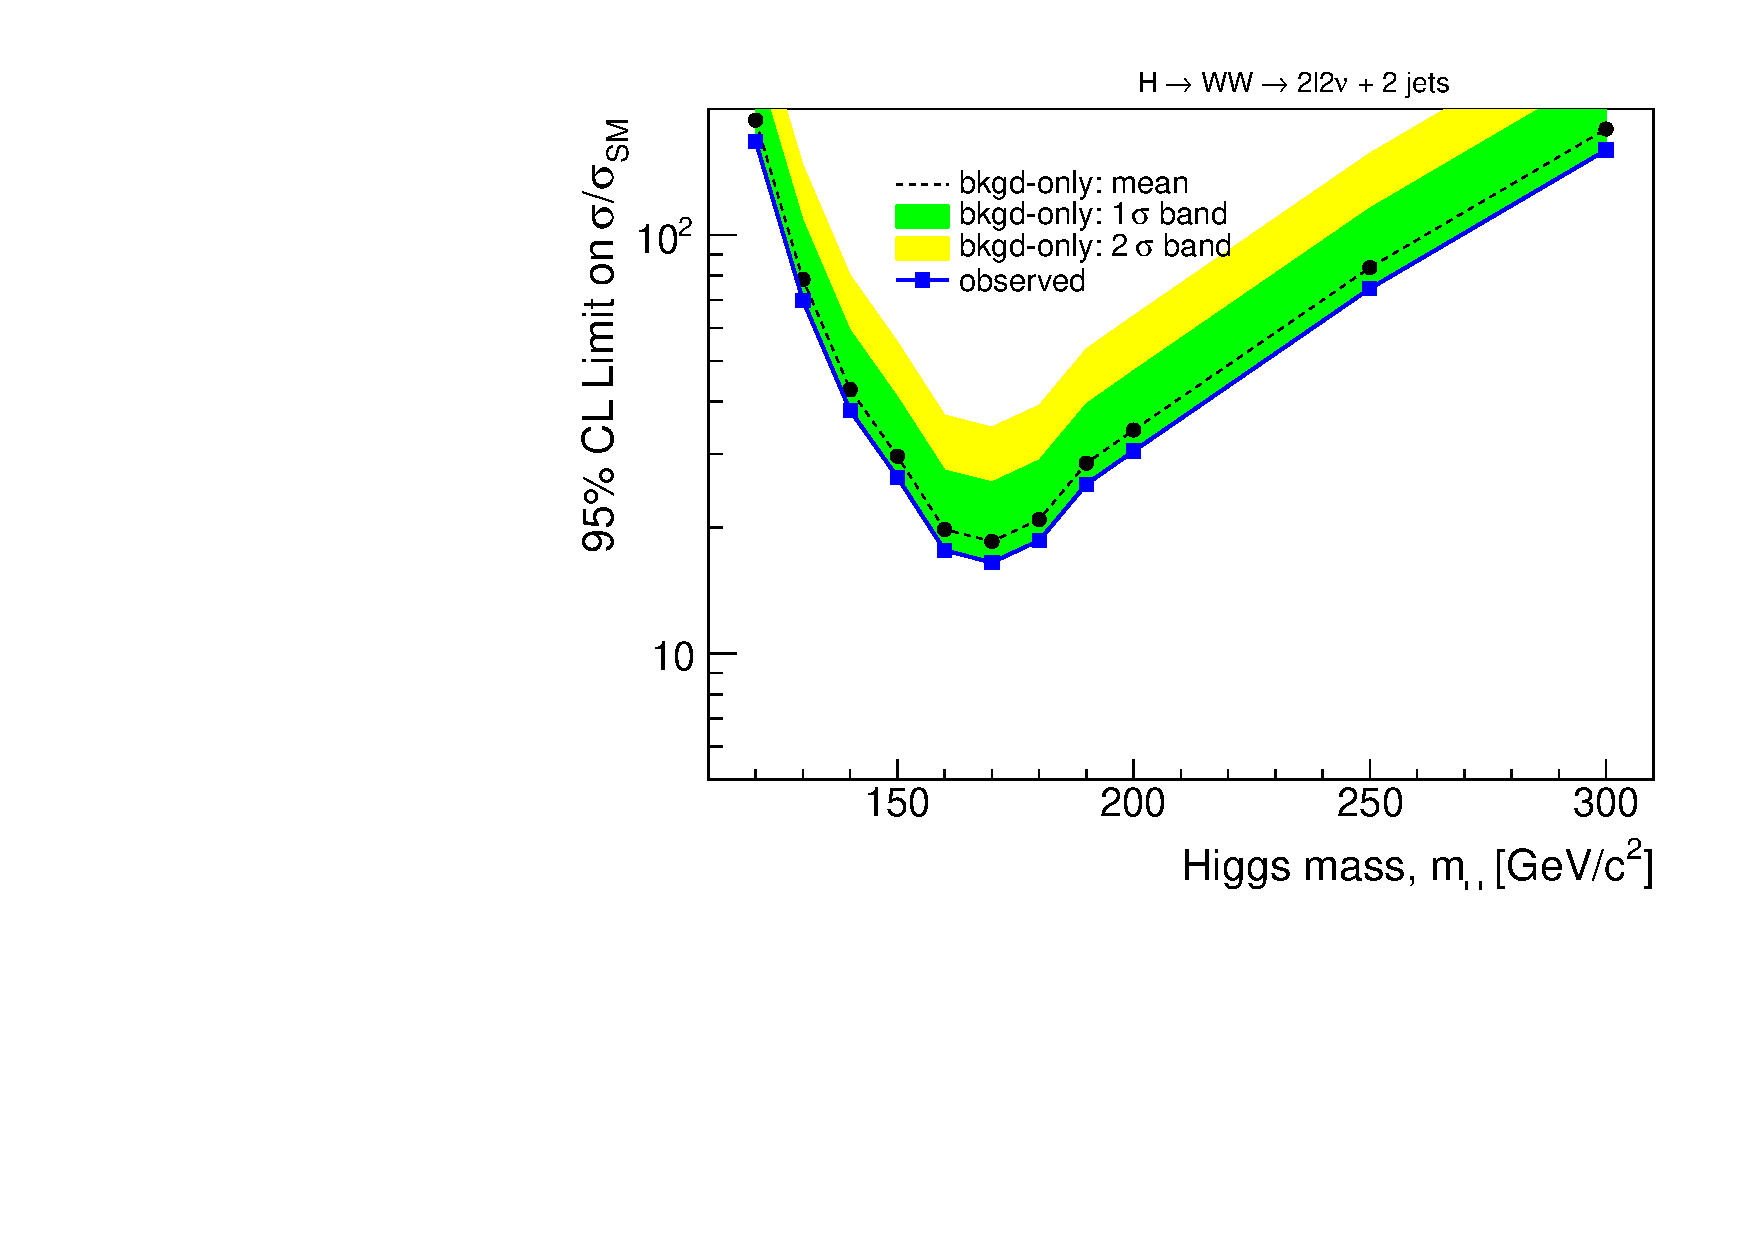
\includegraphics[width=0.49\textwidth]{figures/limits_2j_50pb_cut_1.pdf}
   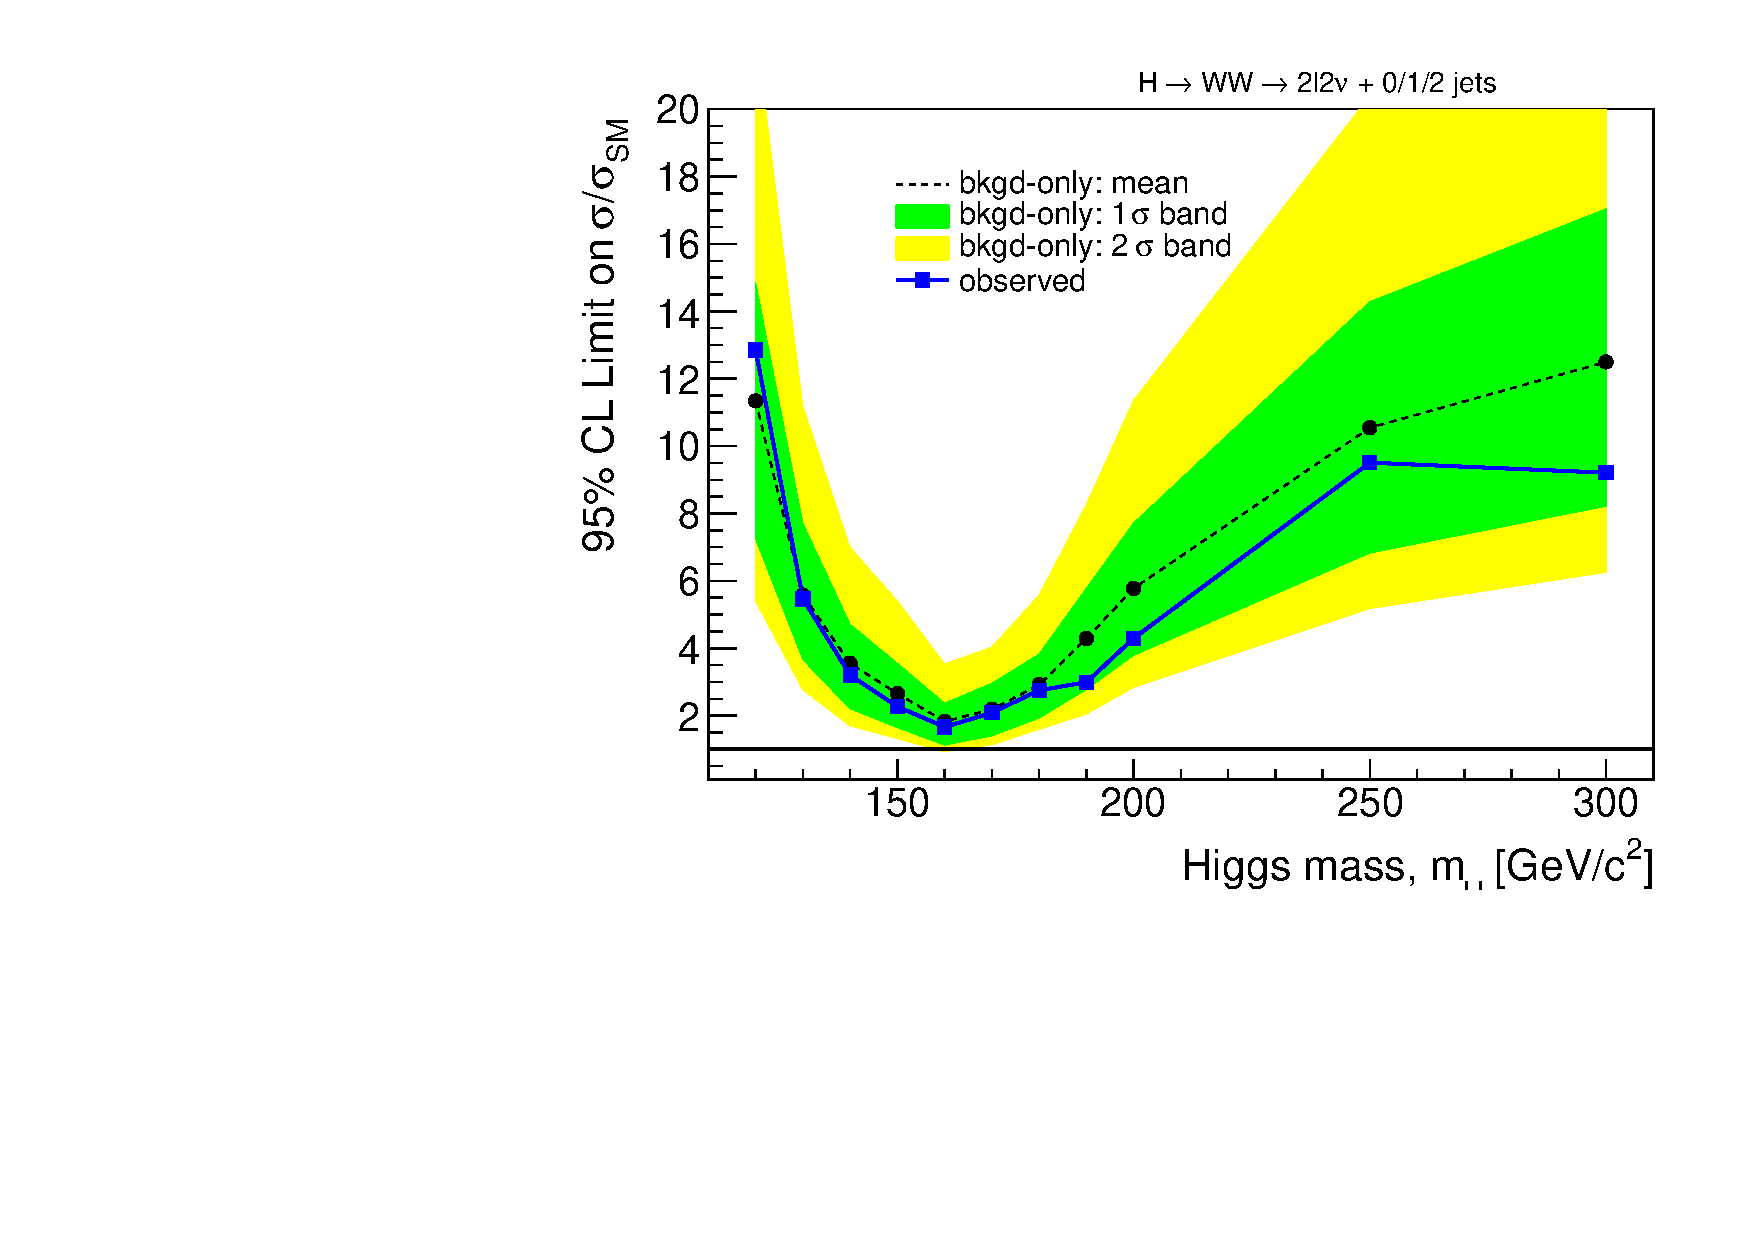
\includegraphics[width=0.49\textwidth]{figures/limits_nj_50pb_cut_1.pdf}
   \caption{Cut based analysis expected upper limits at 95\% C.L. for 49 $\ipb$ of data. Top left plot 
   is the result for the 0-jet bin, top right plot is the result for the 1-jet bin, bottom left plot 
   is the result for the 2-jet bin and, bottom right plot is the combined result.}
   \label{fig:cutbase_uls_data}
\end{center}
\end{figure}

\begin{figure}[!htbp]
\begin{center}
   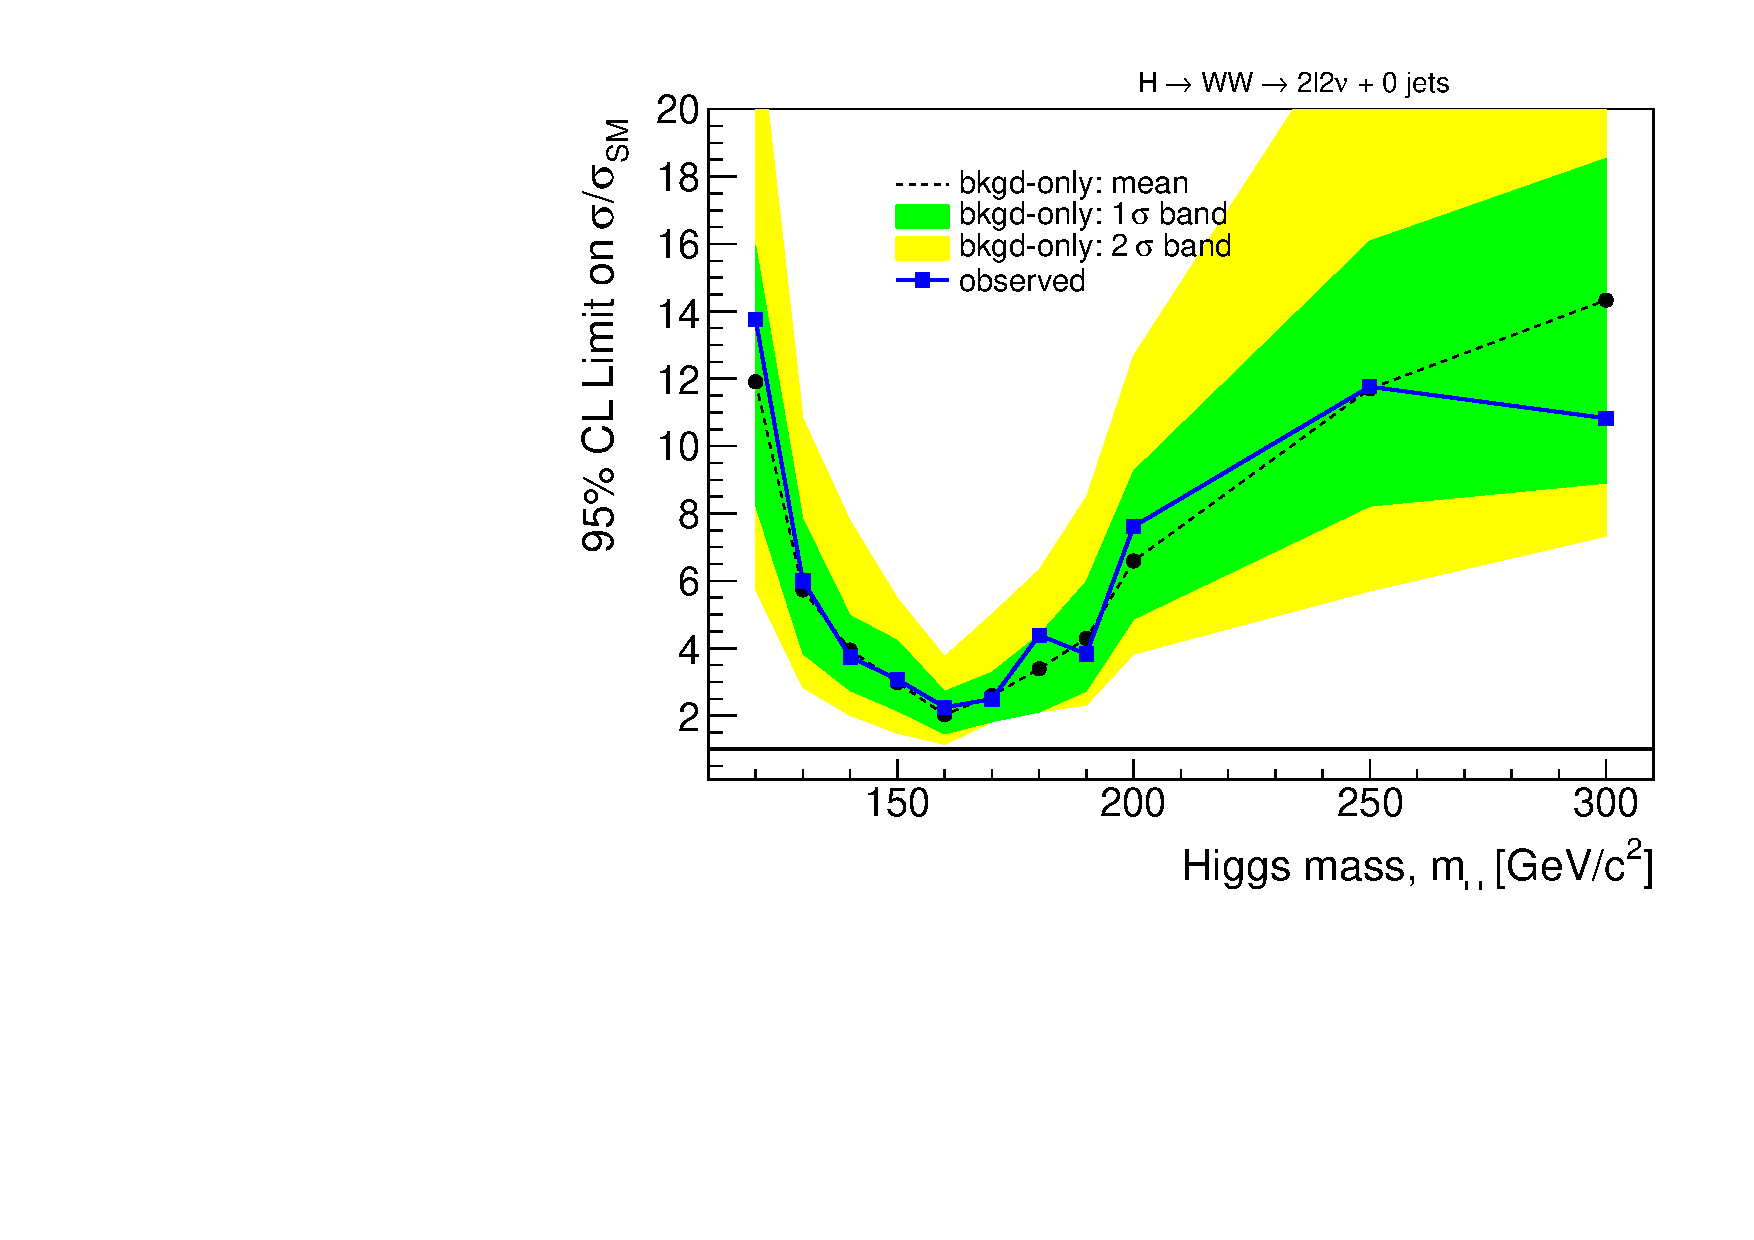
\includegraphics[width=0.49\textwidth]{figures/limits_0j_50pb_mva_1.pdf}
   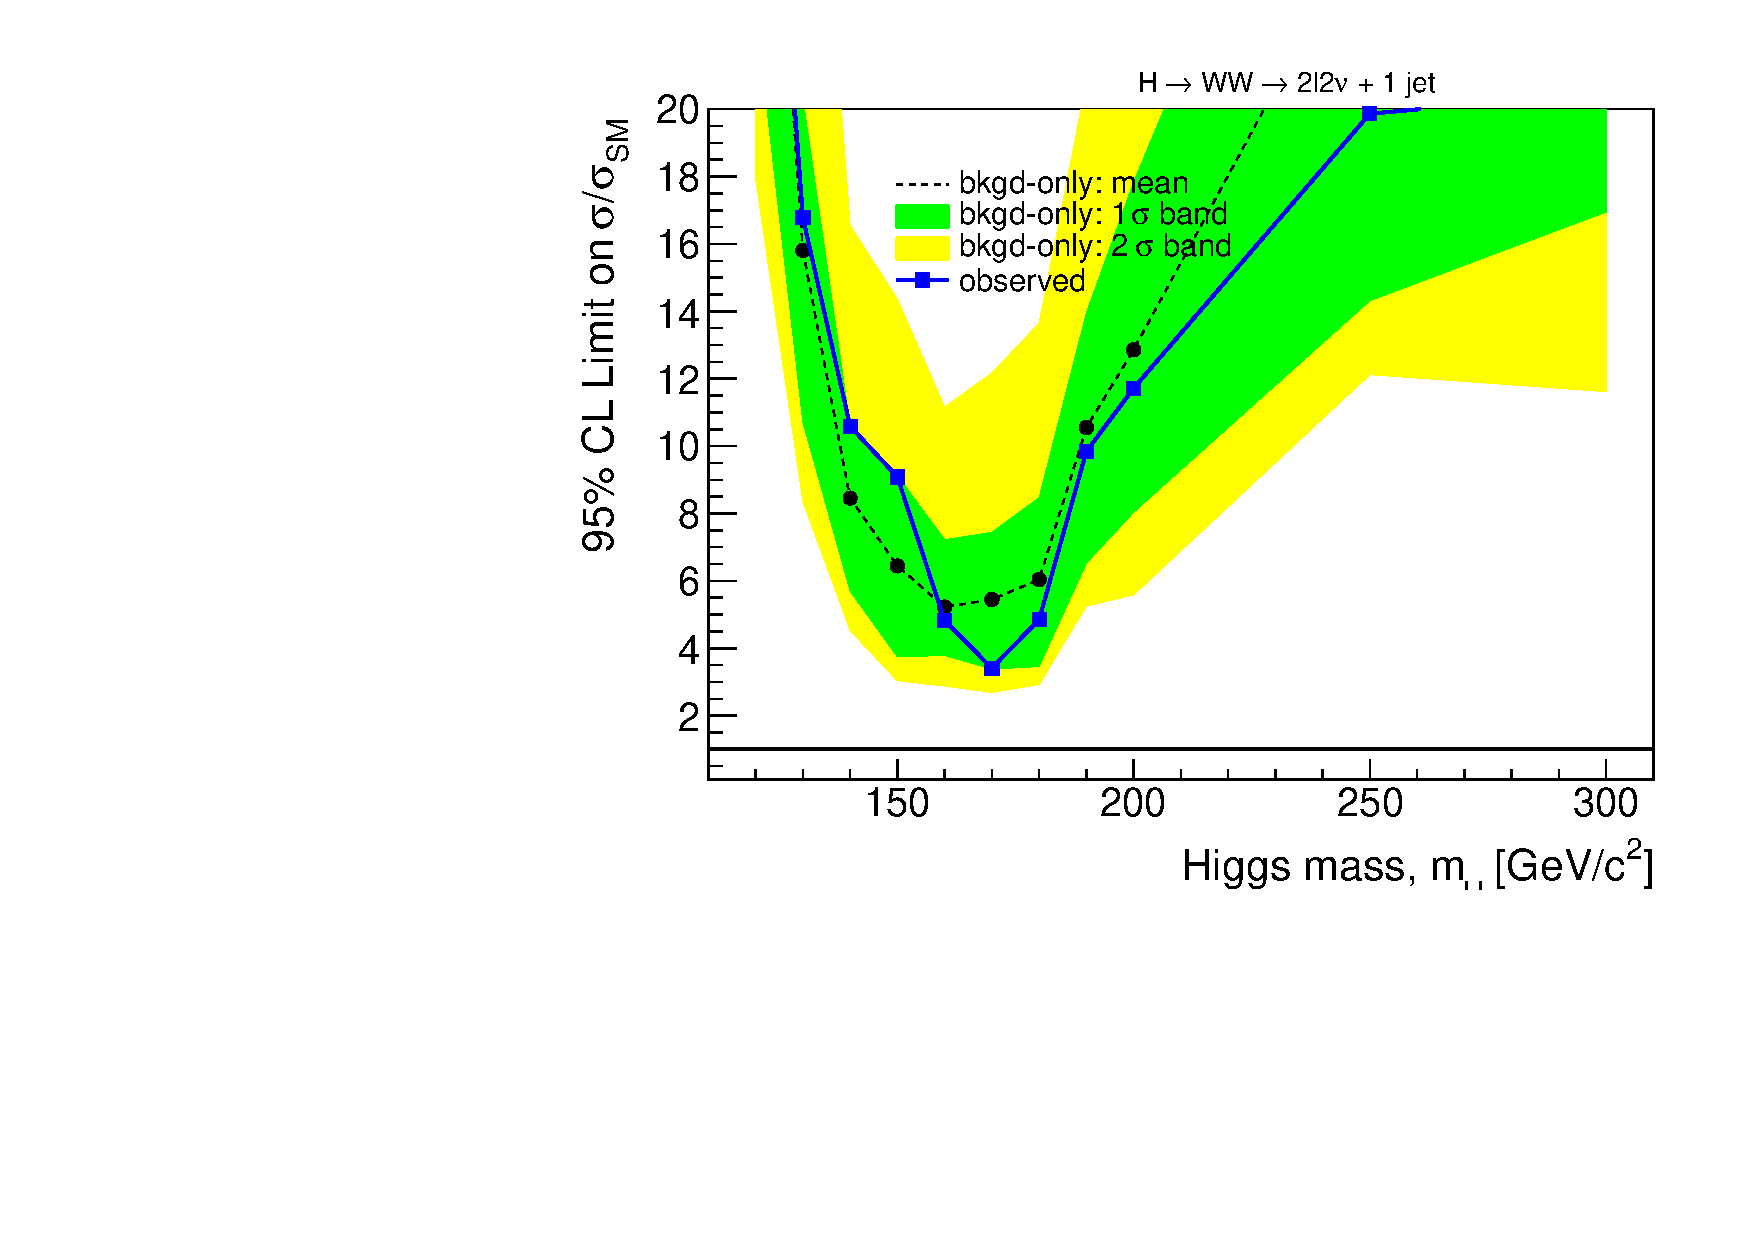
\includegraphics[width=0.49\textwidth]{figures/limits_1j_50pb_mva_1.pdf}
   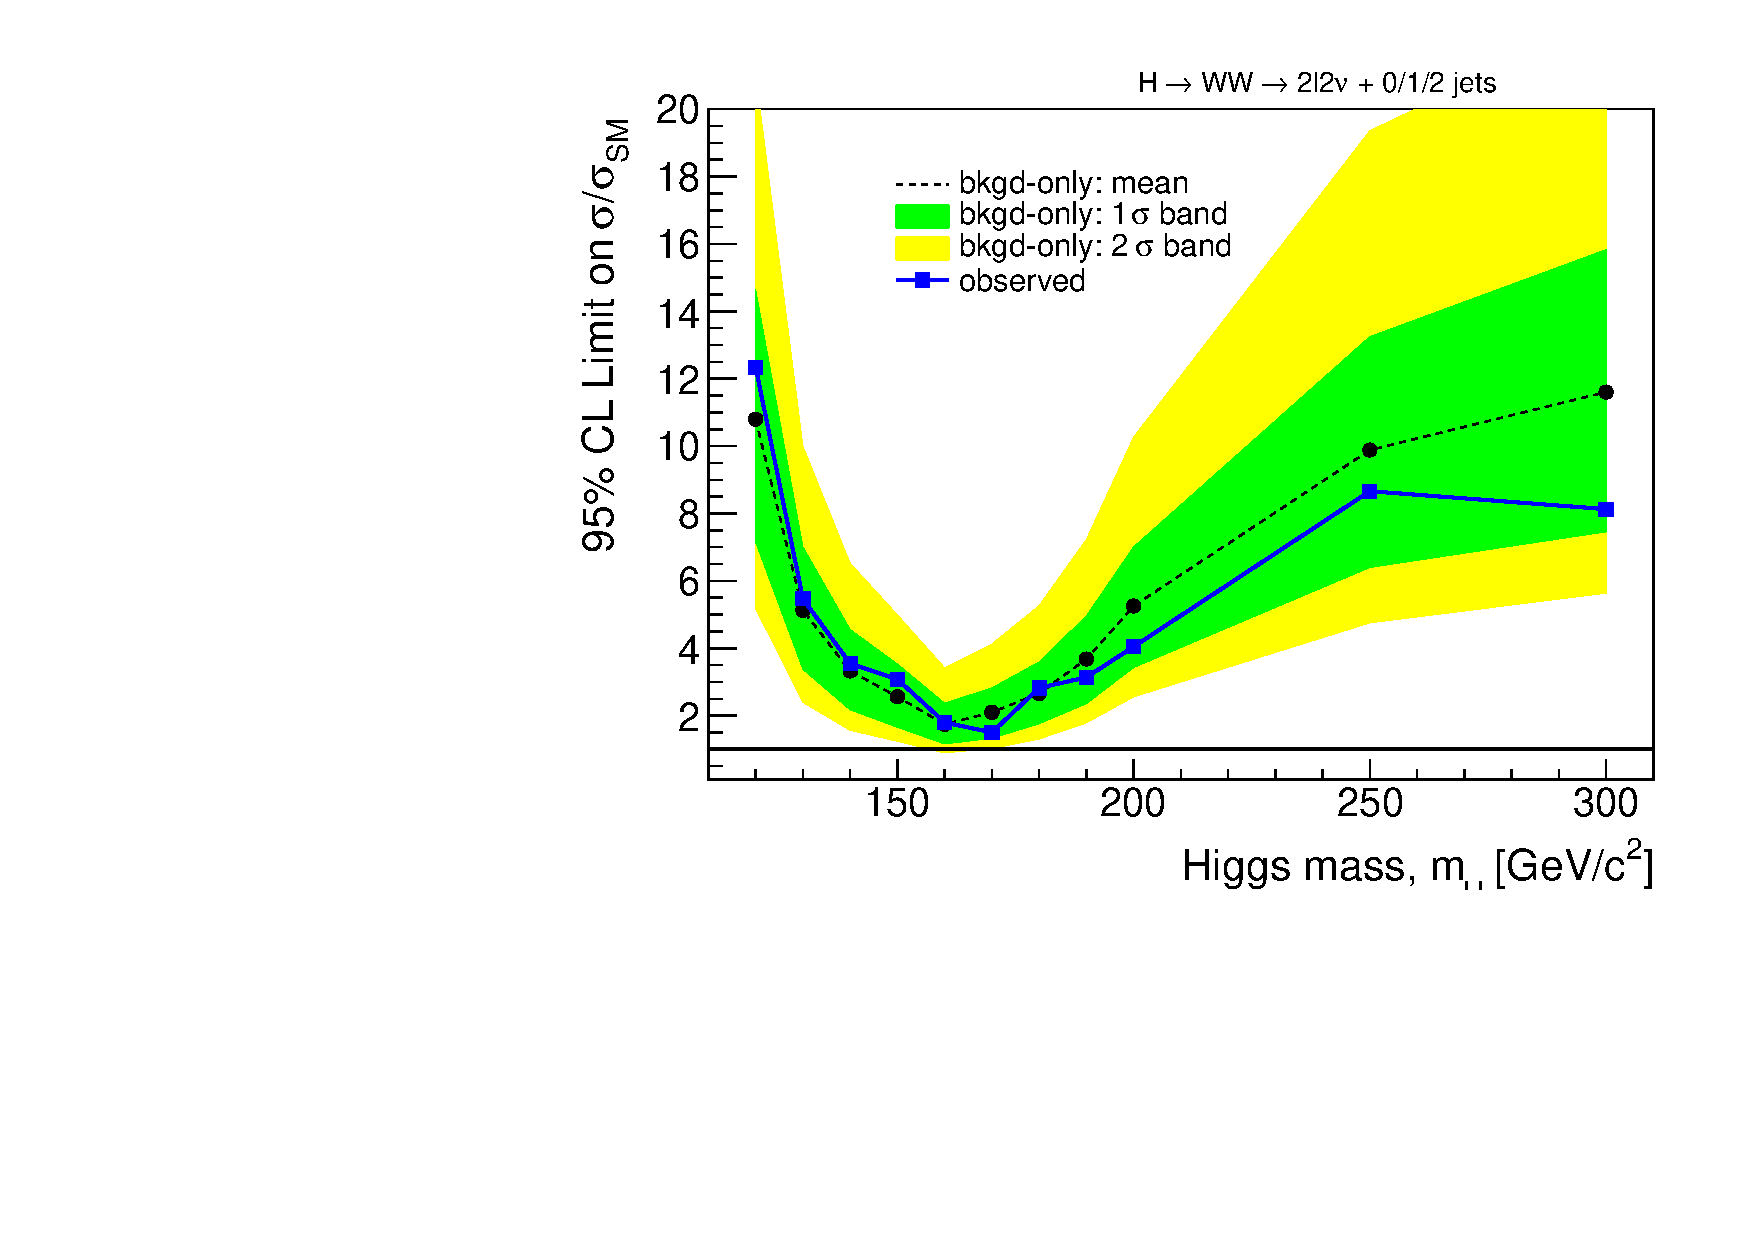
\includegraphics[width=0.49\textwidth]{figures/limits_nj_50pb_mva_1.pdf}
   \caption{Multivariate analysis expected upper limits at 95\% C.L. for 49 $\ipb$ of data. Top left plot 
   is the result for the 0-jet bin, top right plot is the result for the 1-jet bin and, 
   bottom right plot is the combined result.}
   \label{fig:mvabase_uls_data}
\end{center}
\end{figure}
